\chapter*{Executive Summary}
Multirotor drones are cheap, small, quick, and agile, enabling innovation across many industries in the past decade. In a similar manner, Software Defined Radios are bringing cheap, reconfigurable radios to market. The combination of the highly maneuverable drone with the software defined radio allows for a unique style of triangulation. Instead of taking samples in parallel from multiple devices, samples are taken at multiple points sequentially from one device. This is only possible with a quickly moving device like a drone and targets that move slowly, such as a stationary Wi-Fi access point or lost hiker in the woods. \par

By researching prior art, it was determined that similar projects have been conducted on these individual technologies, but none with them combined. Examples of prior art are \cite{path_planning_snr_mqp} and \cite{sdr_localization_mqp}. The former project elaborated on the use of a UAV to perform multi-agent path planning, image processing and communication to conduct search and rescue operations. The latter project implemented a localization system using a Software Defined Radio based upon an IEEE 802.11b communications platform. Consequently, the research conducted in this project will be the foundation of future development. \par

The implementation of this system can be separated into the following blocks: coding framework, drone control, spectrum sensing, spectrum localization, and transmission to ground. These blocks are described in Figure \ref{fig:sys_diagram}. Due to the modular platform's independence from the drone, the coding framework describes the actions of the system dependent on the state of the drone. These actions are condensed into the states of sensing, rotation, on-board computing, and transmission to ground. The states are processed by the Single Board Computer (SBC) component of the system. Most commercial drones operate at 2.4 GHz, the targeted sensing spectrum for this project. This poses an issue because of the possibility of drone control signals interfering with the signals that the SDR is receiving. To address this, the wireless cards were replaced so that these drones can operate at 5 GHz, a different frequency to the targeted spectrum. To conduct this spectrum sensing, the SBC had to be interfaced with the Universal Software Radio Peripheral hardware driver (UHD) to the Ettus board. This required knowledge of how these libraries worked and how information is parsed in order to perform matched filtering. The board also was interfaced with a Global Positioning System (GPS) that determines the device's location. This provides the necessary base coordinates for localization. To improve accuracy, the GPS was passed through a Kalman Filter to smooth the location information. GNU Radio was used to transmit this information and receive at a ground station over 900MHz. \par 
\begin{figure}[ht!]
    \centering
    \includegraphics[width=0.70\textwidth]{img/drone_framework}
    \caption{Block diagram of system operation. Split into drone control and SBC coding framework.}
    \label{fig:sys_diagram}
\end{figure}

The outcome of this project was a 3DR Solo drone capable of carrying the platform to detect nearby wireless signals. The prototype is shown in Figure \ref{fig:drone_and_box_exec} below.
\begin{figure}[ht!]
    \centering
    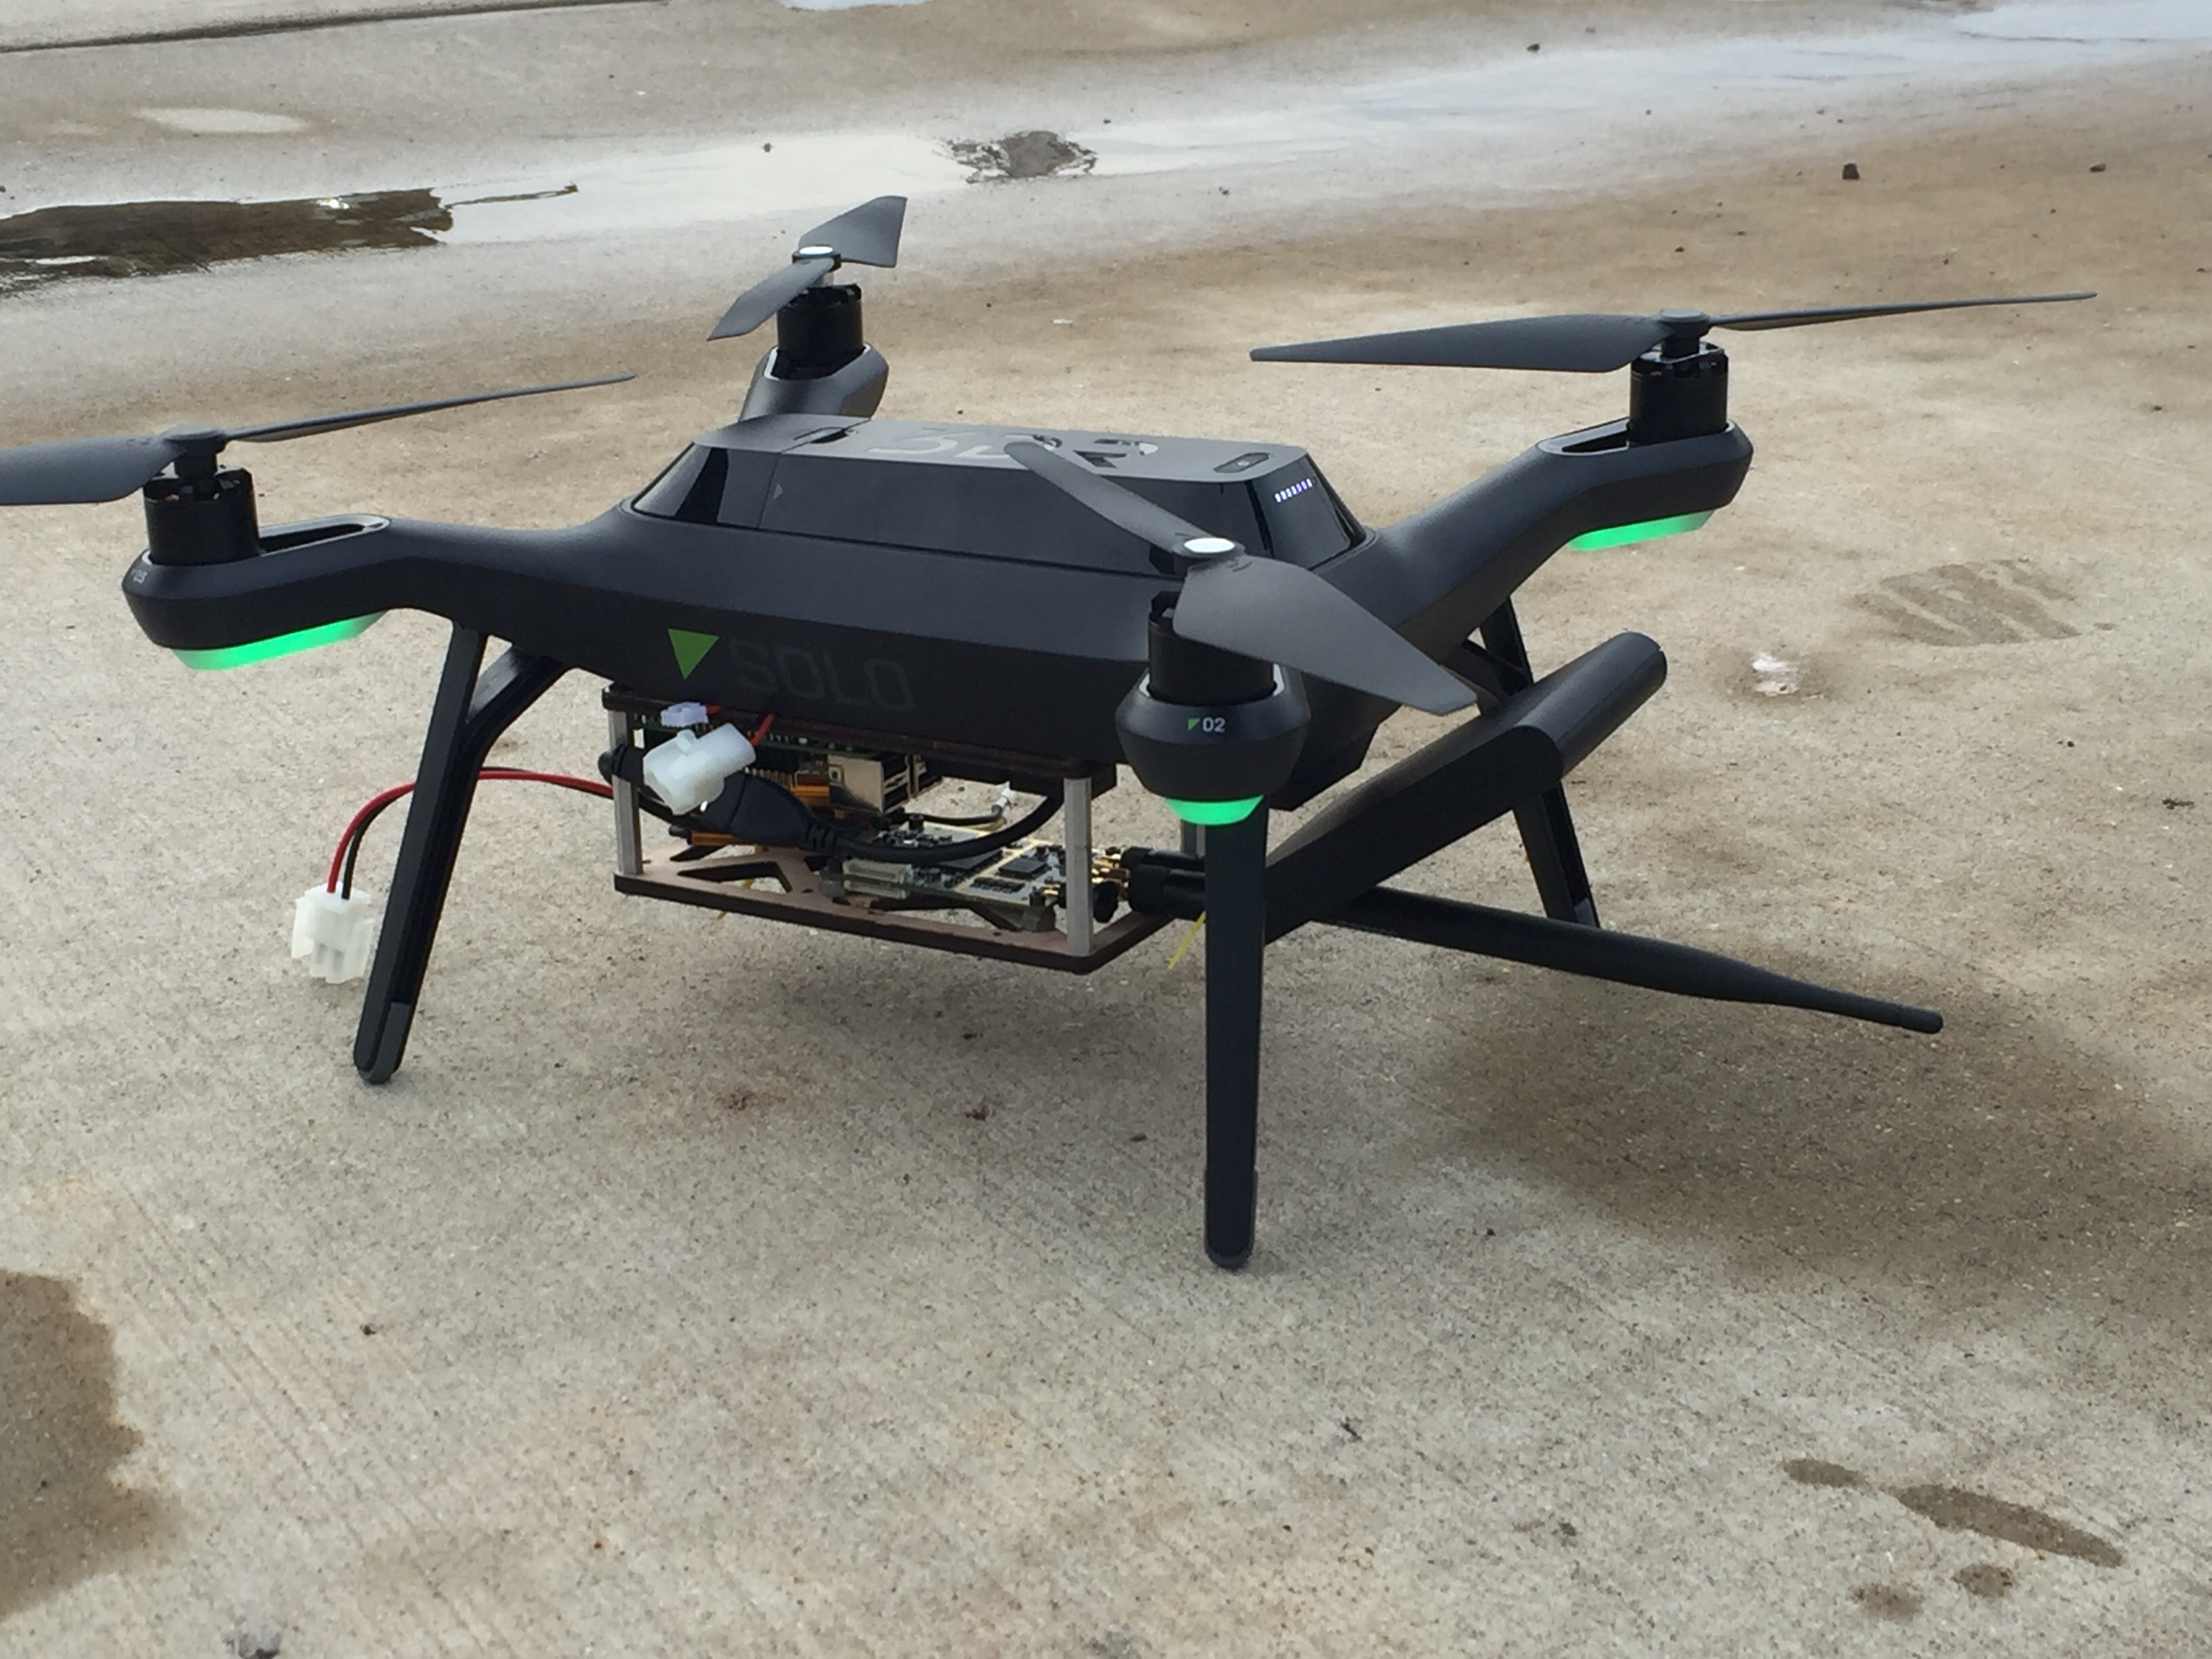
\includegraphics[width=0.70\textwidth]{img/drone_and_box.jpg}
    \caption{The complete system mounted on the drone. In flight testing was done with this setup.}
    \label{fig:drone_and_box_exec}
\end{figure}
The received data corresponds well with the tests conducted. However, the obtained GPS values are not reliable enough to accurately localize the signal, despite the modeling of the Kalman Filter. Once the GPS values are reliable enough, the Python script coded will be able to map and determine the most likely point of origin of the signal. The transmission to ground is viable in lab scenarios but has not been fully integrated into the system when flown due to a malfunctioning device. \par